% vim: set tw=78 sts=2 sw=2 ts=8 aw et ai:
\documentclass[12pt]{article}

\usepackage[paper=a4paper, top=2cm, bottom=3cm, left=2.5cm, right=2.5cm]{geometry}

\usepackage{ucs}
\usepackage[utf8x]{inputenc}
\usepackage[english]{babel}
%\usepackage{hyperref}	  % use \url{http://$URL} or \href{http://$URL}{Name}
\usepackage{underscore}	  % underscores need not be escaped
\usepackage{subfigure}
\usepackage{verbatim}
\usepackage{float}

% Support for including graphics
\usepackage{graphicx}
\DeclareGraphicsExtensions{.pdf,.png,.jpg}

\title{Grand Report Title}

\author{Catalina Macalet, Sorin Dumitru\\
Automatic Control and Computers Faculty\\
University Politehnica of Bucharest\\
Splaiul Independenței nr. 313, Bucharest, Romania \\
\emph{\{catalina.macalet,sorin.dumitru\}@cti.pub.ro}}

\date{\today}

\begin{document}

\maketitle

\begin{abstract}
% vim: set tw=78 sts=2 sw=2 ts=8 aw et ai:
In this paper we report our research on some existing wireless network
simulators, namely NS-2, J-sim and TOSSIM and introduce \codename the 
wireless network simulator which we will develop hereafter, presenting its 
features and going into details regarding the architectural design and implementation.

All the surveyed simulators were not intended from the beginning to be
used for WSN simulations but rather modified later in order to simulatet WNSs, 
\codename it is to be used only 
for WSNs simulations, its design and
implementation being focused on taking the best decision for an accurate WSN
simulation. It will benefit from the experience of the already implemented
simulators using some of their key features and improving some others but
it will also bring new features.


\end{abstract}

Keywords:
\begin{itemize}
  \item WSN
  \item Routing protocols
  \item NS-2/J-Sim/TOSSIM
\end{itemize}

\section{Introduction}
\label{sec:introduction}
% vim: set tw=78 sts=2 sw=2 ts=8 aw et ai:

Wireless sensor networks consist of numerous autonomous sensors that are
capable of monitoring the environment in which they are placed with various
sensors. Such a network would be usefull for monitoring different things such
asas polution levels
in a city or poisonous gases or might be able to sense vibrations in order 
to predict an earthquake. 

A wireless sensor network will contain many nodes, anywhere from a couple of
hundred sensors to several thounds of nodes. Each of these nodes has one or
more sensors incorporated for getting data from the environment, the number of
sensors is limited
by the size and power consumption. Sensors also have a microcontroller 
to process the data from the sensor and a transceiver to be able send to some 
sink-node the data it collected. They are usually powered by some sort of battery 
although solar cells and capacitors have also been used.

Each sensor collects data from its location and sends it to the base station,
from where data from the whole network can be collected. A usual WSN is
presented in \figref{img:wsn}. It is very power
consuming to send data over long distances as the transceiver will need to
amplify the power more so this should be avoided if possible by sending data to
closer nodes. From this need of preserving the power 
arised a need of routing protocols for these
networks: instead of sending data directly to the base station, the nodes
group in an hierarchical way so that each node will send data to a cluster
head that is very close, which then sends it to the base station or to a higher
order cluster head.

\fig{img/WSN.pdf}{img:wsn}{WSN}
%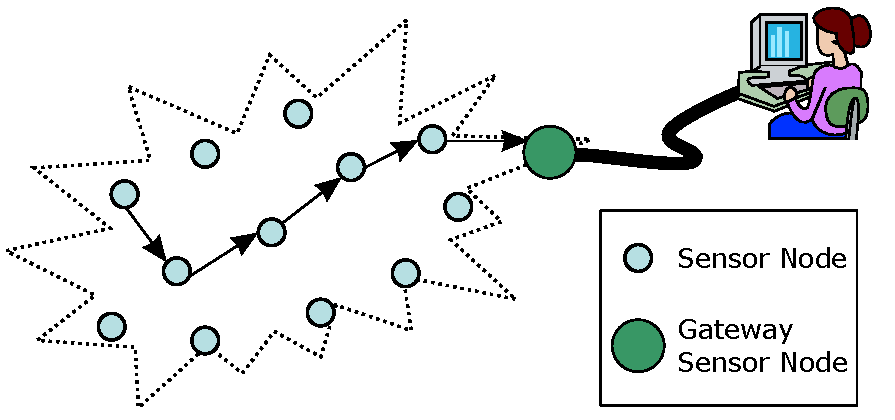
\includegraphics{img/WSN.pdf}

In this paper we will present some of the existing wireless network
simulators emphasizing what we believe to be their strenghts and weaknesses. 
In section NS-2 we discuss about NS-2 simulator, in section J-sim we present
J-sim and then we take a look at TOSSIM simulator. Based on these observations
we introduce in section \codename, the WSN simulator we will implement which
encompasses most of these simulators' strenghts and adds some new features
for wireless network simulators.


\section{Architecture}
\label{sec:architecture}
\label{subsec:architecture}

The simulator we will be building will have a modular design. Each type
of component, a battery or a sensor, will a have a template containing a
very basic implementation of it. For example a transceiver template will
have a template consisting of the send() and recv() methods, but more
usefull implementations will be built on this to take into account the
environment and power consumption. On top of this template many different
implementations may be derived; for example a lithium-ion battery or a solar
powered one. Each component will provide an access interface for other components
(a sensor might have a read_data() interface) and they will not depend on other 
components. This way we will be able to simulate a wide range of platforms by
combining different components in different slots.

All the activity on one node will be coordinated by a CPU component. This will provide
an API to the routing protocol running on the node for activities such as allocating memory 
and sending and receiving packets. To simulate a slower node, the code running on the 
node will be ran using the \textit{ptrace} system call. The protocol will set in the beginning
breakpoints at every point in the program and the parent process(the node) will limit
its speed based on a configured value. We do not see any reasons to have more than one
type of CPU so only one will be available, but its performance and available memory
will be configurable.

Data through the network will not come only from the routing protocol, but sensors on the 
node will be able to generate realistic data that will accurately model the normal load
on such a network. This is important in order to see how protocols behave under load 
because some of them work by aggregating data.

It is important to be able to gather information from the network(number of packets sent
or received, battery life, power consumption per device) so there will be a central agent
responsible for gathering this information. Each component will send the statistics gathered
by them to the agent who will be able to present them in a more usefull form (bars and pies).


\section{Implementation}
\label{sec:implementation}
% vim: set tw=78 sts=2 sw=2 ts=8 aw et ai:

Proper implementation is proper.


\section{Experimental Setup}
\label{sec:setup}
% vim: set tw=78 sts=2 sw=2 ts=8 aw et ai:

In order to define recursion, one must first define recursion.


\section{Scenarios and Results}
\label{sec:results}
% vim: set tw=78 sts=2 sw=2 ts=8 aw et ai:

The end justifies the means.


\section{Conclusion and Further Work}
\label{sec:conclusion}
% vim: set tw=78 sts=2 sw=2 ts=8 aw et ai:

While the simulators investigated in this paper are very useful, we believe
that there is room for improvement. Most of them are generic simulators
adapted for simulating wireless sensor networks. 
We believe that a simulator built from the beginning, having in mind that it
will be used for wireless sensors, will increase its usability and make it
possible for it to be useful in more circumstances.
We propose the following plan to build the simulator described above in a couple
of phases.
We will begin by fully designing the component architecture and basic node
structure. We will build template components and create the necessary framework to integrate them 
into a sensor node. Next we will create the necessary framework for the nodes
to communicate. 
After being able to simulate a wireless sensor network, we will implement some
routing protocols, such as LEACH and TEEN, and based on the results of the
simulation of these protocols, we will determine \codename's performance.
The final step is integrating the environment simulation into the simulator.
We will augment the simulator with environment simulation as described in the paper.
%\begin{itemize}
%  \item Component architecture and basic node structure. We will build
%  template components and create the necessary framework to integrate them
%  into a sensor node.
%  \item Comunication between nodes. Create the neccessary framework to make
%  two nodes communicate.
%  \item Implement some routing procols. To evaluate our simulator we will
%  implement some routing procols(LEACH, TEEN) in it and see it's performance
%  \item Environment simulation. Will augment the simulator with environment
%  simulation as described in the paper.
%\end{itemize}


\section*{Acknowledgment}
\label{sec:acknowledgment}

The authors would like to thank XYZ for their support and dedication.

\bibliographystyle{abbrv}
\bibliography{my-report}

\end{document}
